\section{Introduction}
\label{sec:introduction}

\subsection{Motivation}
\label{sec:motivation}

Computer information analysis is the only known approach to work with huge amount of data produced every day. In any field of human work there is data and there are tasks of analyzing it. The topic of this thesis combines two areas of data computing: information visualization and biological data processing.

There are many datasets for analysis in biology. This thesis is intended to make a visualization tool for genes and gene relations in order to help biologists with their work. Data for processing was provided by the Plant Bioinformatics Group of Leibniz Institute of Plant Genetics and Crop Plant Research (IPK), Germany. Data consists of Gene Ontologies and hierarchical clustering which are are both important tools in biology and medicine for high-throughput data study.

To help analyzing this data the following approaches are desired: visualizing the data set in the context of a ontology (such as the Gene Ontology) and in the context of data clustering. There is no solutions that deals with combined visualization of ontology (DAG) and an hierarchical clustering (tree) of one data set. The aim of this work is creation of a new visualization approach and is implementation in order to provide a useful tool for biologists in their everyday research work.

The result of this work is a base of the research paper -- \textsf{Ilir Jusufi, Andreas Kerren, Vladyslav Aleksakhin, and Falk Schreiber. Visualization of Mappings between the Gene Ontology and Cluster Trees. Conference on Visualization and Data Analysis 2012 (EI-107) Part of IS&T/SPIE Electronic Imaging 2012 (Jan 22-26, 2012) VDA 2012 Dates: January 23-25, 2012.}

\subsection{Thesis Collaboration}
This project is the result of collaboration between ISOVIS research group (Head: Prof. Dr. Andreas Kerren~\cite{Kerren}) of Linn\ae us University at V\"axj\"o, Sweden, and Plant Bioinformatics Group (Head: Prof. Dr. Falk Schreiber~\cite{Schreiber}) of Leibniz Institute of Plant Genetics and Crop Plant Research (IPK), Germany.


ISOVIS research group is focused on the exploration analysis and visualization of large information data in Software Engineering, Geography, or Biology. There are several different techniques for information visualization, one of them is widely used in the research is Human-Centered Visualization. This kind of visualization combines different research areas: Information Visualization, Scientific Visualization, Human-Computer Interaction, Data Mining, Information Design, Graph Drawing, and Computer Graphics.


As said on official page of Plant Bioinformatic Group: ,,The research group focuses on modeling, analysis, simulation and visualization of biological networks in the context of plant biological problems. Our aim is the development of methods and software tools for the analysis of complex biological networks. Therefore we integrate, process and analyze data from different areas of genome, proteome and
metabolome research and present the results in a user-friendly way. The emphasis is on the linkage of experimental data about expression profiles and metabolite patterns with metabolic and regulatory networks. The data and complex connections are modeled using graphs. We are developing graph (network) analysis and interactive visualization methods to discover network properties and to make the data easily accessible to the user. A subsequent step is to use the data for the simulation of metabolic and regulatory networks.''~\cite{PBG}


\subsection{Thesis Outline}
\label{sec:structure}

Section~\ref{sec:introduction} explains the problem, thesis purpose and collaboration. Section~\ref{sec:background} presents the results of the related work, where relevant research efforts in the fields of Bioinformatic, Information Visualization and Bio Visualization were explored in connection to the thesis work. Section~\ref{sec:algorithm} covers the following topics: visualization complexity and describes the goals, description of the input data and mapping between graphs. Section~\ref{sec:solution} describes attempt to the visualization solution, the solution for Cluster Ananlysis tree and the visualization solution for Gene Ontology visualization technique. One of the biggest section in the report is Section~\ref{sec:implementation} that determines the requirements, use cases, and proposes the architecture for thesis application.
Additionally in Section~\ref{sec:solution} describes the input data format overview, overview of the different graph file formats, implementation details, architecture of the system, used libraries, project management tools. Technical details of the visualization algorithms are explained in Sections~\ref{sec:cluster} and~\ref{sec:go}. Last part of the report is Section~\ref{sec:conclusion} that describes problems and future work.

\section{Background}
\label{sec:background}


\subsection{Information Visualization}
\label{sec:infovis}

The field of computer-based information visualization draws on ideas from several intellectual traditions: computer science, psychology, semiotics, graphic design, cartography, and art.
The two main threads of computer science relevant for visualization are computer graphics and human-computer interaction.
The areas of cognitive and perceptual psychology offer important scientific guidance on how humans perceive visual information.
A related conceptual framework from the humanities is semiotics, the study of symbols and how they are convey meaning.
Design, as the name suggests, is about the process of creating artifacts well- suited for their intended purpose.
Cartographers have a long history of creating visual representations that are carefully chosen abstractions of the real world.
Finally, artists have refined methods for conveying visual meaning in sub-disciplines ranging from painting to cinematography.

Information visualization has gradually emerged over the past fifteen years as a distinct field with its own research agenda.
The distillation of results from areas with other goals into specific prescriptive advice helping us to design and evaluate visualization systems is nontrivial.
Although these traditions have much to offer, effective synthesis of such knowledge into a useful methodology.

The standard argument for visualization is that exploiting visual processing can help people explore or explain data. We have an active field of study because the design challenges are significant and not fully understood. Questions about visual encoding are even more central to information visualization than to scientific visualization.
The subfield names grew out of an accident of history, and have some slightly unfortunate connotations when juxtaposed:
information visualization is not unscientific, and scientific visualization is not uninformative.
The distinction between these two is still not agreed on by all, but the definition used here is that information visualization hinges on finding a spatial mapping of data that is not inherently spatial,
whereas scientific visualization uses a spatial layout that is implicit in the data.

\begin{figure}[h!]
\centering
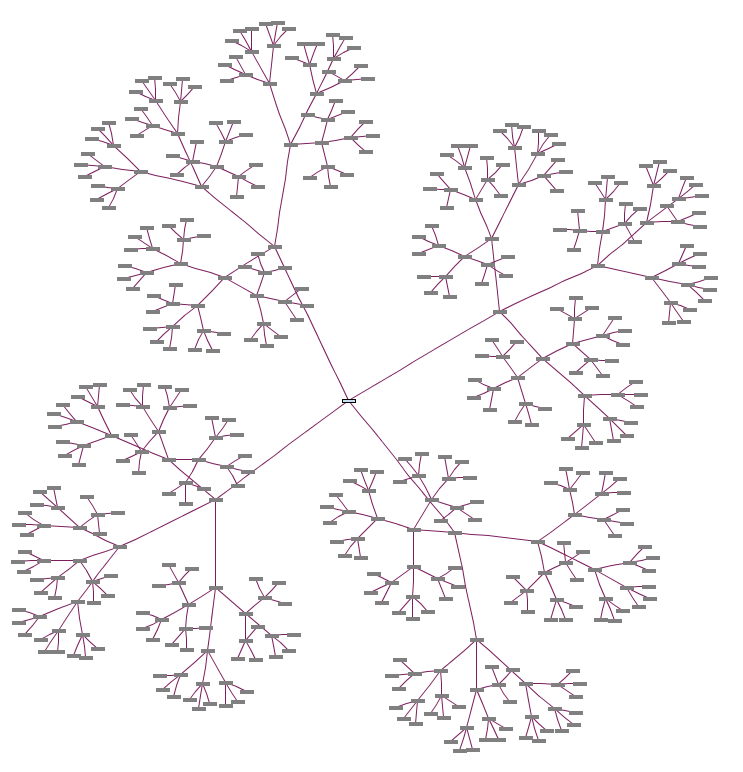
\includegraphics[scale=0.3]{pictures/Tree_graph_example.png}
\caption{Sample visualisation of the tree graph}
\label{fig:tree_graph_example}
\end{figure}

,,Graph drawing or Graph layout, as a branch of graph theory, applies topology and geometry to derive two-dimensional representations of graphs.
A drawing of a graph is basically a pictorial representation of an embedding of the graph in the plane (generally, with edge intersections allowed),
usually aimed at a convenient visualization of certain properties of the graph in question or of the object modeled by the graph.
Graph drawing is motivated by applications such as Very-large-scale (VLSI)~\cite{VLSI} integration circuit design, social network analysis,
cartography, and bioinformatics, many of which make use of information visualization.''~\cite{Graph_drawing}

There are many methods and approaches to graph visualization. They are all based on various perception qualities of human.
The Radial Dendrograms~\cite{Radial_dendrogram} algorithm is used for results of cluster analysis visualization.

Dendrogram~\cite{Dendrogram} plot is one of the visualization algorithm for hierarchical structures. It illustrating the outcome of decision tree-type clustering in statistics.
Most commonly, dendrograms are drawn in a Cartesian layout, as an upright tree. However, this layout does not make good use of space, it is sparse towards the root and crowded towards the leaf nodes.
The spacing between nodes at different levels in the hierarchy is not uniform, which is due to the shrinking number of nodes from bottom to top. For this reason, long, wide-spanning connecting lines are needed to merge nodes at higher levels.
A better layout in this respect is a polar or a radial layout, where leaf nodes are located on the outer ring and a root is located in the center, as a focal point.
A more uniform node spacing results are leading to a better utilization of space and resulting to a better illustration of the class relationships.
Recently, Barlow and Neville~\cite{Barlow_Neville} presented an empirical user study for tree layouts (with less than 200 leaves) in which they compare some of the major schemes: the organizational chart (a standard drawing of a tree),
the tree ring (basically a pie chart of circular segments), the icicle plot (the cartesian version of the tree ring), and the tree map. According to the measured performance within a group of 15 users,
the three former methods yielded similar results where the icicle plot has a slight advantage. However, given larger number of leaves in our case (1000 and more) and the fact that the tree ring is the most compact of the three winning configurations,
a radial layout seemed to be the most favorable one for our purpose. Radial graph layouts that illustrate hierarchical relationships are very popular, and for the special application of dendrograms.
We know only one other application that uses a radial layout. The recent one by Kreussler and Schumann~\cite{Kreussler_Schumann} that mentioned before, users often would like to focus on certain portions of the display,
while compressing others, without losing context. Fisheye lenses and hyperbolic zooming were proposed to provide these capabilities.
In the context of tree rings Yang, Ward and Rundensteiner~\cite{Yang_Ward} proposed a system in which users may either perform a polar zoom (i.e. expand the width of one or more adjacent rings while reducing others) or
a radial zoom (i.e. expand the arc angle of some adjacent segments while reducing others). More over, users can perform these operations by pinning down one ring or arc segment and dragging another.
A limiting factor here is that users cannot perform both operations simultaneously that can be awkward in certain instances. To address this shortcoming
our application generalizes these concepts by allowing arbitrary warps of the dendrogram domain, i.e. we allow radial and polar zooms simultaneously.


\subsection{Bioinformatics}
\label{sec:bioinformatics}

''In the last few decades, advances in molecular biology and the equipment available for research in this field have allowed the increasingly rapid sequencing of large portions of the genomes of several species.
In fact, to date, several bacterial genomes, as well as those of some simple eukaryotes (e.g., Saccharomyces cerevisiae, or baker's yeast) have been sequenced in full.
The Human Genome Project, designed to sequence all 24 of the human chromosomes, is also progressing. Popular sequence databases, such as GenBank and EMBL, have been growing at exponential rates.
This deluge of information has necessitated the careful storage, organization and indexing of sequence information. Information science has been applied to biology to produce the field called Bioinformatics.


The simplest tasks used in bioinformatics concern the creation and maintenance of databases of biological information.
Nucleic acid sequences (and the protein sequences derived from them) comprise the majority of such databases. While the storage and or organization of millions of nucleotides is far from trivial,
designing a database and developing an interface whereby researchers can both access existing information and submit new entries is only the beginning.
The most pressing tasks in bioinformatics involve the analysis of sequence information''~\cite{Biology}


Here we can find short introduction and history of Bioinformatics: ,,Bioinformatics is the application of information technology to the field of molecular biology.
The term bioinformatics was coined by Paulien Hogeweg in 1978 for the study of informatic processes in biotic systems.
Bioinformatics now entails the creation and advancement of databases, algorithms, computational and statistical techniques, and theory to solve formal and practical problems arising from the management and analysis of biological data.
Over the past few decades rapid developments in genomic and other molecular research technologies and developments in information technologies have combined to produce a tremendous amount of information related to molecular biology.
It is the name given to these mathematical and computing approaches used to glean understanding of biological processes.
Common activities in bioinformatics include mapping and analyzing DNA and protein sequences, aligning different DNA and protein sequences to compare them and creating and viewing 3-D models of protein structures.''~\cite{Bioinformatic}
More resources about Bioinformatic are available here~\cite{Bioinformatic_resources}.
The primary goal of bioinformatics is to increase our understanding of biological processes.
However, its focus on developing and applying computationally intensive techniques (e.g., data mining, machine learning algorithms, and visualization) to achieve this goal sets it apart from other approaches.
Major research efforts in the field include sequence alignment, gene finding, genome assembly, protein structure alignment, protein structure prediction, prediction of gene expression and protein-protein interactions, genome-wide association studies and the modeling of evolution.

\subsection{Gene Ontology}
\label{sec:gene_ontology}

As stated above, there are different knowledge databases for biologic information storage.
Gene Ontology~\cite{GO_website} project is one of the first-rate international projects.
The Gene Ontology, or GO, is a major bioinformatics initiative to unify the representation of gene and gene product attributes across all species.
The aims of the Gene Ontology project are threefold. Firstly, to maintain and further develop its controlled vocabulary of gene and gene product attributes,
secondly, to annotate genes and gene products, and assimilate and disseminate annotation data,
and thirdly, to provide tools to facilitate access to all aspects of the data provided by the Gene Ontology project.
The GO is part of a larger classification effort, the Open Biomedical Ontologies (OBO)~\cite{OBO}.
The Gene Ontology project provides an ontology of defined terms representing gene product properties.
The ontology covers three domains. First is cellular component and the parts of a cell or its extracellular environment.
Second is molecular function and the elemental activities of a gene product at the molecular level, such as binding or catalysis and biological process.
Finally the third are operations or sets of molecular events with a defined beginning and end, pertinent to the functioning of integrated living units: cells, tissues, organs, and organisms. Each GO term within the ontology has a term name, which may be a word or string of words;
a unique alphanumeric identifier; a definition with cited sources; and a name space indicating the domain to which it belongs.
Terms may also have synonyms, which are classed as being exactly equivalent to the term name, broader, narrower, or related; references to equivalent concepts in other databases;
and comments on term meaning or usage. The GO ontology is structured as a directed acyclic graph, where each term has defined relationships to one or more other terms in the same domain, and sometimes to other domains. The GO vocabulary is designed to be species-neutral,
and includes terms applicable to prokaryotes and eukaryotes, single and multicellular organisms.
The GO ontology is not static, therefore additions, corrections and alterations are suggested by and solicited from members of the research and annotation communities, as well as by those directly involved in the GO project.
For example, an annotator may request a specific term to represent a metabolic pathway, or a section of the ontology may be revised with the help of community experts.
Suggested edits are reviewed by the ontology editors and implemented where appropriate.


\subsection{Clustering}
\label{sec:clustering}

,,Data clustering (or just clustering), also called cluster analysis, segmentation analysis, taxonomy analysis, or unsupervised classification,
is a method of creating groups of objects, or clusters, in such a way that objects in one cluster are very similar and objects in different clusters are quite distinct.
Data clustering is often confused with classification, in which objects are assigned to predefined classes. In data clustering, the classes are also to be defined.''~\cite{data_clustering_book}


Clustering algorithms can be applied in many fields. For instance:

\begin{itemize}
\item Marketing: finding groups of customers with similar behavior given a large database of customer data that contains their properties and past buying records;
\item Biology: classification of plants and animals given their features;
\item Libraries: book ordering;
\item Insurance: identifying groups of motor insurance policy holders with a high average claim cost, identifying frauds;
\item City-planning: identifying groups of houses according to their house type, value and geographical location;
\item Earthquake studies: clustering observed earthquake epicenters in order to identify dangerous zones;
\item WWW: document classification clustering web log data to discover groups of similar access patterns.
\end{itemize}